\selectlanguage{english}

\chapter{Algorithms} \label{app1}

\minitoc

\section{Reject inference methods} \label{app1:reject}

\subsection{Fuzzy Augmentation} \label{fuzzy}

Fuzzy Augmentation can be found in \cite{economix}; it is the following procedure:
\begin{enumerate}
\item Construct Scorecard "Known Good Bad" (KGB) $\hat{\gls{bth}}_\f$ with financed clients' data (Figure \ref{fuzzy:sfig1})
\item Calculate $p(1|x,\hat{\theta}_{\text{f}})$ for rejects (Figure \ref{fuzzy:sfig2})
\item Infer rejected client $i$ as good with weight $p(1|x,\hat{\theta}_{\text{f}})$ and as bad with weight {\begin{sloppypar} $1-p(1|x,\hat{\theta}_{\text{f}})$ (Figures \ref{fuzzy:sfig2} and \ref{fuzzy:sfig3}) \end{sloppypar} }
\item Calibrate a new scorecard with the ‘‘augmented'' dataset (Figure \ref{fuzzy:sfig4})
\end{enumerate}

\begin{table}
\caption{\label{fuzzyexample} Example of implementation of the Fuzzy Augmentation method on a small dataset}
{\setlength{\parindent}{0cm}
\begin{multicols}{4}
\small

\begin{subfigure}[t]{0.22\textwidth}
\begin{center}
\begin{adjustbox}{max width=0.95\textwidth}
\begin{tabular}{l l}
\toprule
\textbf{${\bm{y}}_{\text{f}}$} & \textbf{${\bm{x}}_{\text{f}}$}\\
\midrule
1 & 0.562 \\
1 & 0.910 \\
0 & 0.430 \\
\bottomrule
\end{tabular}
\end{adjustbox}
\end{center}

\subcaption{Scorecard $\hat{\gls{bth}}_\f$ on financed loans}
\label{fuzzy:sfig1}
\end{subfigure}

\columnbreak

\begin{subfigure}[t]{0.22\textwidth}
\begin{center}
\begin{adjustbox}{max width=0.95\textwidth}
\begin{tabular}{l l l}
\toprule
\textbf{Weight} & \textbf{$\hat{\bm{y}}_{\text{nf}}$} & \textbf{${\bm{x}}_{\text{nf}}$}\\
\midrule
0.68 & 1 & 0.347 \\
0.10 & 1 & 0.140 \\
0.35 & 1 & 0.295 \\
\bottomrule
\end{tabular}
\end{adjustbox}
\end{center}

\caption{Inferred good not financed loans and their weights}
\label{fuzzy:sfig2}
\end{subfigure}

\columnbreak

\begin{subfigure}[t]{0.22\textwidth}
\begin{center}
\begin{adjustbox}{max width=0.95\textwidth}
\begin{tabular}{l l l}
\toprule
\textbf{Weight} & \textbf{$\hat{\bm{y}}_{\text{nf}}$} & \textbf{${\bm{x}}_{\text{nf}}$}\\
\midrule
0.32 & 0 & 0.347 \\
0.90 & 0 & 0.140 \\
0.65 & 0 & 0.295 \\
\bottomrule
\end{tabular}
\end{adjustbox}
\end{center}

\caption{Inferred bad not financed loans and their weights}
\label{fuzzy:sfig3}
\end{subfigure}

\columnbreak

\begin{subfigure}[t]{0.22\textwidth}
\begin{center}
\begin{adjustbox}{max width=0.95\textwidth}
\begin{tabular}{l l l}
\toprule
\textbf{Weight} & \textbf{${\bm{y}}$} & \textbf{${\bm{x}}$}\\
\midrule
1 & 0 & 0.562 \\
1 & 1 & 0.910 \\
1 & 0 & 0.430 \\
0.68 & 1 & 0.347 \\
0.10 & 1 & 0.140 \\
0.35 & 1 & 0.295 \\
0.32 & 0 & 0.347 \\
0.90 & 0 & 0.140 \\
0.65 & 0 & 0.295 \\
\bottomrule
\end{tabular}
\end{adjustbox}
\end{center}
\caption{Fuzzy augmented learning dataset}
\label{fuzzy:sfig4}
\end{subfigure}

\end{multicols}
}
\end{table}

 Clearly:

 \[ \forall j = 1, \ldots, d, \: \frac{\partial \sum_{i=n+1}^{m+n} \sum_{y_i = 0}^{1} p_{\hat{\gls{bth}}_\f}(\gls{y}_i| \gls{bx}_i)\ln (p_{\gls{bth}}(\gls{y}_i| \gls{bx}_i))}{\partial \theta_j} = 0 \Leftrightarrow \theta = \hat{\theta}_{\text{f}} \]

 Such that:
 \[\argmax_{\theta \in \Theta}  \sum_{i=n+1}^{m+n} \sum_{y_i = 0}^{1} p_{\hat{\theta}_{\text{f}}}(y_i| x_i)\ln (p_\theta(y_i| x_i)) = \hat{\theta}_{\text{f}}\]

 And finally:
 \[\argmax_{\theta \in \Theta} \ell(\theta;{\bm{x}},{\bm{y}}_{\text{f}},{\bm{y}}_{\text{nf}}) = \argmax_{\theta \in \Theta} \ell(\theta;{\bm{x}},{\bm{y}}_{\text{f}}) = \hat{\theta}_{\text{f}}\]

 To conclude, this method will not change the estimated parameters of any discriminant model, asymptotically and with a finite set of observations, regardless of any assumption on the missingness mechanism or the true model hypothesis. In other words, Fuzzy Augmentation has no effect on the $\gls{KL}$ divergence, making this method useless because it is no different than the financed clients model.


\subsection{Reclassification} \label{reclassification}

Reclassification can be found in \cite{RI6}, also sometimes referred to as extrapolation as in \cite{banasik}; it is the following procedure:
\begin{enumerate}
\item Construct Scorecard "Known Good Bad" (KGB) $\hat{\gls{bth}}_{\text{f}}$ with financed clients' data (Figure~\ref{reclass:sfig1})
\item Calculate $p_{\hat{\theta}_{\text{f}}}(1|\gls{bx})$ for rejects
\item Infer default status of rejected client $i$ if $p_{\hat{\theta}_{\text{f}}}(1|\gls{bx}) > \text{threshold}$; typically threshold $=0.5$ (Figure~\ref{reclass:sfig2})
\item Calibrate a new scorecard with the ‘‘augmented'' dataset (Figure~\ref{reclass:sfig3})
\end{enumerate}

\begin{table}
\caption{\label{reclassexample} Example of implementation of the Reclassification method on a small dataset}
{\setlength{\parindent}{0cm}
\begin{multicols}{3}

\begin{subfigure}[t]{0.31\textwidth}
\begin{center}
\begin{adjustbox}{max width=\textwidth}
\begin{tabular}{l l}
\toprule
\textbf{${\bm{y}}^{\text{f}}$} & \textbf{${\bm{x}}^{\text{f}}$}\\
\midrule
1 & 0.562 \\
1 & 0.910 \\
0 & 0.430 \\
\bottomrule
\end{tabular}
\end{adjustbox}
\end{center}

\caption{Development of scorecard $S^{\text{f}}$ on financed clients}
\label{reclass:sfig1}
\end{subfigure}


\columnbreak

\begin{subfigure}[t]{0.31\textwidth}
\begin{center}
\begin{adjustbox}{max width=\textwidth}
\begin{tabular}{l l l}
\toprule
\textbf{$p(1|x,\hat{\theta}^{\text{f}})$} & \textbf{$\hat{\bm{y}}^{\text{nf}}$} & \textbf{${\bm{x}}^{\text{nf}}$}\\
\midrule
0.68 & 1 & 0.347 \\
0.10 & 0 & 0.140 \\
0.35 & 0 & 0.295 \\
\bottomrule
\end{tabular}
\end{adjustbox}
\end{center}

\caption{We force $y^{\text{nf}}=1$ if $\text{logit}(S^{\text{f}}(x)) \geq 0.5$}
\label{reclass:sfig2}
\end{subfigure}

\columnbreak

\begin{subfigure}[t]{0.31\textwidth}
\begin{center}
\begin{adjustbox}{max width=\textwidth}
\begin{tabular}{l l}
\toprule
\textbf{${\bm{y}}$} & \textbf{${\bm{x}}$}\\
\midrule
0 & 0.562 \\
1 & 0.910 \\
0 & 0.430 \\
1 & 0.347 \\
0 & 0.140 \\
0 & 0.295 \\
\bottomrule
\end{tabular}
\end{adjustbox}
\end{center}
\caption{Reclassified learning dataset}
\label{reclass:sfig3}
\end{subfigure}

\end{multicols}
}
\end{table}


\subsection{Augmentation} \label{augmentation}

Augmentation can be found in \cite{RI6}. It is also documented as a ``Re-Weighting method'' by \cite{saporta,banasik,economix}.

\begin{enumerate}
\item Construct Scorecard "Accept Reject" (ACRJ) $\hat{\gls{phi}}$ with financed clients' data on target variable $Z$ (Figure~\ref{augment:sfig1})
\item Create $K$ score bands $B_1, \ldots, B_K$ according to $p_{\hat{\gls{phi}}}(\gls{z} | \gls{bx})$
\item Compute in each score band $\hat{p}(\text{f}|x \in B_k) = \dfrac{|B_k|}{|\gls{F}|}$ (Figure~\ref{augment:sfig2})
\item Construct a new scorecard on target variable Good/Bad with financed clients' data re-weighted (Figure~\ref{augment:sfig3})
\end{enumerate}

\begin{table}
\caption{\label{augmentexample} Example of implementation of the Augmentation method on a small dataset}
{\setlength{\parindent}{0cm}
\begin{multicols}{3}

\begin{subfigure}[t]{0.31\textwidth}
\begin{center}
\begin{adjustbox}{max width=0.95\textwidth}

\begin{tabular}{l l l}
\toprule
\textbf{${\bm{y}}$} & \textbf{${\bf{z}}$} & \textbf{Score-band}\\
\midrule
1 & \text{f} & 1 \\
1 & \text{f} & 1 \\
0 & \text{f} & 1 \\
NA & \text{nf} & 1 \\
NA & \text{nf} & 1 \\
NA & \text{nf} & 1 \\
... & ... & ... \\
\bottomrule
\end{tabular}
\end{adjustbox}
\end{center}

\caption{Calculation of $K$ score-bands on the ACRJ score}
\label{augment:sfig1}
\end{subfigure}

\columnbreak

\begin{subfigure}[t]{0.31\textwidth}
\begin{center}
\begin{adjustbox}{max width=0.95\textwidth}

\begin{tabular}{l l l}
\toprule
\textbf{Score-band} & \textbf{Weight}\\
\midrule
1 & 2 \\
... & ... \\
K & 1.1 \\
\bottomrule
\end{tabular}
\end{adjustbox}
\end{center}

\caption{Aggregate the data to estimate the inverse of the probability of being accepted in each score band}
\label{augment:sfig2}
\end{subfigure}

\columnbreak

\begin{subfigure}[t]{0.31\textwidth}
\begin{center}
\begin{adjustbox}{max width=0.95\textwidth}

\begin{tabular}{l l l l}
\toprule
\textbf{Weight} & \textbf{Score-band} & \textbf{${\bm{y}}$} & \textbf{${\bm{x}}$}\\
\midrule
2 & 1 & 1 & 0.123 \\
2 & 1 & 0 & 0.432 \\
2 & 1 & 1 & 0.562 \\
... & ... & ... & ... \\
1.1 & K & 0 & 0.962 \\
1.1 & K & 0 & 0.812 \\
\bottomrule
\end{tabular}
\end{adjustbox}
\end{center}

\caption{Merge weights and data on financed clients to construct the new scorecard}
\label{augment:sfig3}
\end{subfigure}
\end{multicols}
}
\end{table}

\subsection{Twins} \label{Twins}

The Twins Method is an internal method at \gls{cacf} documented in~\cite{groupe} (confidential) where Figure~\ref{fig:twins} is given; it consists in the following procedure:
\begin{enumerate}
\item Develop KGB (Known Good/Bad) scorecard $\hat{\gls{bth}}_\f$ on financed clients' data predicting $\gls{bby}_\f$ given $\gls{bbx}_\f$ (Figure~\ref{twins:sfig1})
\item Develop ACRJ (Accept/Reject) scorecard $\hat{\gls{phi}}$ on all applicants predicting $\mathbf{\bm{z}}$ given $\gls{bbx}$; this gives us $\hat{\gls{phi}}$ (Figure~\ref{twins:sfig2})
\item Develop a scorecard on financed clients' data predicting $\gls{bby}_\f$ based solely on $(1,\gls{bbx}_f)' \hat{\gls{bth}}_\f$ and $(1,\gls{bbx}_f)' \hat{\gls{phi}}$; this gives us $\hat{\theta}^{\text{twins}}$ (Figure~\ref{twins:sfig3})
\item Calculate $p_{\hat{\gls{bth}}^{\text{twins}}}(1 | \gls{bx})$ on rejected applicants and reintegrate them twice in the training dataset like we did with Fuzzy Augmentation in Section \ref{fuzzy} (Figure~\ref{twins:sfig4})
\item Develop a new scorecard on all applicants' data
\end{enumerate}

\begin{figure}
\centering
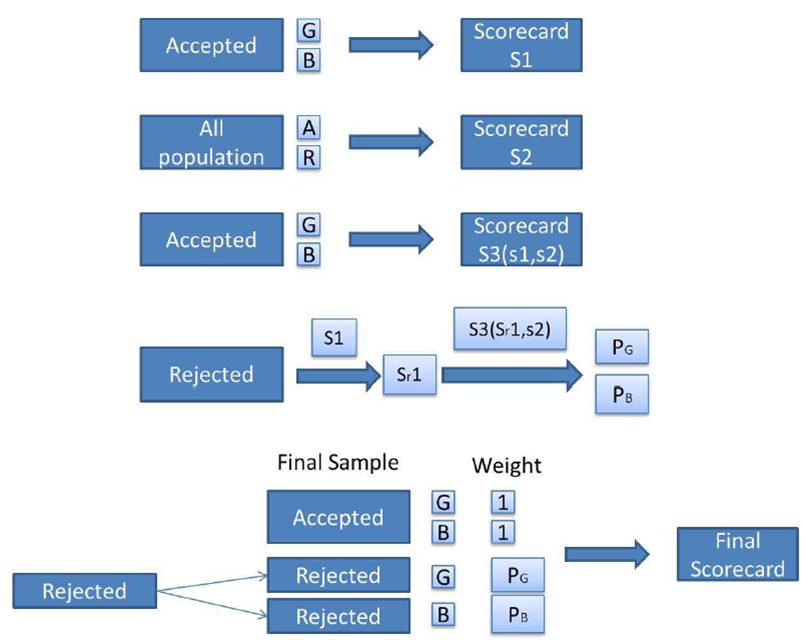
\includegraphics[width=0.5\textwidth]{figures/appendix/processusTwins.png}
\caption{The accompanying Figure of the Twins method in the internal documentation.}
\label{fig:twins}
\end{figure}

\begin{table}
\caption{\label{twins} Example of implementation of the Twins method on a small dataset}
{\setlength{\parindent}{0cm}
\begin{multicols}{4}

\begin{subfigure}[t]{0.22\textwidth}
\begin{center}
\begin{adjustbox}{max width=0.95\textwidth}
\begin{tabular}{l l l}
\toprule
\textbf{${\bm{y}}$} & \textbf{${\bm{x}}$}\\
\midrule
1 & 0.562 \\
1 & 0.910 \\
0 & 0.430 \\
NA & 0.361 \\
NA & 0.402 \\
NA & 0.294 \\
\bottomrule
\end{tabular}
\end{adjustbox}
\end{center}

\caption{Development of scorecard $\hat{\gls{bth}}_\f$ on financed clients}
\label{twins:sfig1}
\end{subfigure}

\columnbreak

\begin{subfigure}[t]{0.22\textwidth}
\begin{center}
\begin{adjustbox}{max width=0.95\textwidth}
\begin{tabular}{l l l}
\toprule
\textbf{${\bm{z}}$} &  \textbf{${\bm{x}}$} \\
\midrule
\text{f} & 0.562 \\
\text{f} & 0.910 \\
\text{f} & 0.430 \\
\text{nf} & 0.361 \\
\text{nf} & 0.402 \\
\text{nf} & 0.294 \\
\bottomrule
\end{tabular}
\end{adjustbox}
\end{center}

\caption{Development of a scorecard $\hat{\gls{phi}}$ on all clients}
\label{twins:sfig2}
\end{subfigure}

\columnbreak

\begin{subfigure}[t]{0.22\textwidth}
\begin{center}
\begin{adjustbox}{max width=0.95\textwidth}
\begin{tabular}{l l l}
\toprule
\textbf{${\bm{y}}$} & \textbf{$(1,\gls{bbx}_f)' \hat{\gls{bth}}_\f$} & \textbf{$(1,\gls{bbx}_f)' \hat{\gls{phi}}$}\\
\midrule
1 & 1.3 & 2.5\\
1 & 3.1 & 4.5 \\
0 & -0.3 & 0.4 \\
NA & -1.2 & -0.5 \\
NA & -0.4 & 0.3 \\
NA & -2.0 & -2.5 \\
\bottomrule
\end{tabular}
\end{adjustbox}
\end{center}

\caption{Development of a new scorecard on financed clients}
\label{twins:sfig3}
\end{subfigure}

\columnbreak

\begin{subfigure}[t]{0.22\textwidth}
\begin{center}
\begin{adjustbox}{max width=0.95\textwidth}
\begin{tabular}{l l l}
\toprule
\textbf{Weight} & \textbf{$\hat{\bm{y}}_{\text{nf}}$} & \textbf{${\bm{x}}_{\text{nf}}$}\\
\midrule
1 & 1 & 0.562 \\
1 & 1 & 0.910 \\
1 & 0 & 0.430 \\
0.64 & 0 & 0.361 \\
0.73 & 0 & 0.402 \\
0.44 & 0 & 0.294 \\
0.36 & 1 & 0.361 \\
0.27 & 1 & 0.402 \\
0.37 & 1 & 0.294 \\
\bottomrule
\end{tabular}
\end{adjustbox}
\end{center}

\caption{Inference for not financed clients}
\label{twins:sfig4}
\end{subfigure}

\end{multicols}
}
\end{table}

Following notations introduced in Chapter~\ref{chap2}, we have:
\[ \ell(\gls{bth};(\bm{1},\gls{bbx})' \hat{\gls{phi}}, (\bm{1},\gls{bbx})' \hat{\gls{bth}}_\f, \gls{bby}) = \sum_{i=1}^{n} \ln(p_{\gls{bth}}(y_i | (1, \gls{bx}_i)' \hat{\theta}_{\text{f}}, (1, \gls{bx}_i)' \hat{\gls{phi}})).\]
We can rewrite $\ell(\gls{bth};(\bm{1},\gls{bbx})' \hat{\gls{phi}}, (\bm{1},\gls{bbx})' \hat{\gls{bth}}_\f, \gls{bby})$ by remarking that the logit of $p_{\gls{bth}}(y_i | (1, \gls{bx}_i)' \hat{\theta}_{\text{f}}, (1, \gls{bx}_i)' \hat{\gls{phi}})$ is a linear combination of $\bm{x}$.
%: $\ell(\gls{bth};(\bm{1},\gls{bbx})' \hat{\gls{phi}}, (\bm{1},\gls{bbx})' \hat{\gls{bth}}_\f, \gls{bby}) = \ell(\theta;\gls{bbx}^{\text{f}}, \gls{bby}^{\text{f}})$ where $\begin{cases}
%\gls{bth} = (\theta_0,\theta_1,\theta_2). \\
%\theta_j = \delta_1 \hat{\theta}_{\text{f}j} + \delta_2 \hat{\zeta}_{j} \text{ for } 1 \leq j \leq d. \\
%\theta_0 = \delta_0 + \delta_1 \hat{\theta}_{\text{f}0} + \delta_2 \hat{\zeta}_{0}.
%\end{cases}$
We know that $\hat{\gls{bth}}^{\text{f}} \in \argmax_{\gls{bth} \in \Theta} \ell(\gls{bth};\gls{bbx}^{\text{f}},\gls{bby}^{\text{f}})$ so that under the identifiability assumption, this method will give the same results as $\hat{\gls{bth}}^{\text{f}}$. In terms of $\gls{KL}$ divergence and as for Fuzzy Augmentation, this method is useless because it is no different than the financed clients model.

\subsection{Parcelling} \label{Parceling}

Parcelling is a process of reweighing according to the probability of default by score-band that is adjusted by the credit modeler. It has been documented in \cite{saporta,banasik,RI6}, as well as in~\cite{groupe} where Figure~\ref{fig:parceling} is given.

\begin{enumerate}
\item Construct Scorecard "Known Good Bad" (KGB) $\hat{\gls{bth}}_\f$ with financed clients' data (Figure~\ref{parcel:sfig1})
\item Create $K$ score bands $B_1, \ldots, B_K$ according to $p_{\hat{\gls{bth}}_\f}(1 | \gls{bx})$.
\item Compute the observed default rate for each band $T(k) = \dfrac{|\text{Bad financed in } B_k|}{|B_k|}$, $1 \leq k  \leq K$.
\item Infer for each band the not financed default rate $U(k) = \epsilon_k T(k)$ where $\epsilon_1 > \ldots > \epsilon_k > \ldots > \epsilon_K > 1$ (Figure~\ref{parcel:sfig2}).
\item Reintegrate 2 times each rejected applicant from $B_k$ with weight $U(k)$ as bad and weight $1-U(k)$ as good, like the Fuzzy Augmentation method in Section \ref{fuzzy} (Figure~\ref{parcel:sfig3}).
\item Construct the final scorecard.
\end{enumerate}

\begin{figure}
\centering
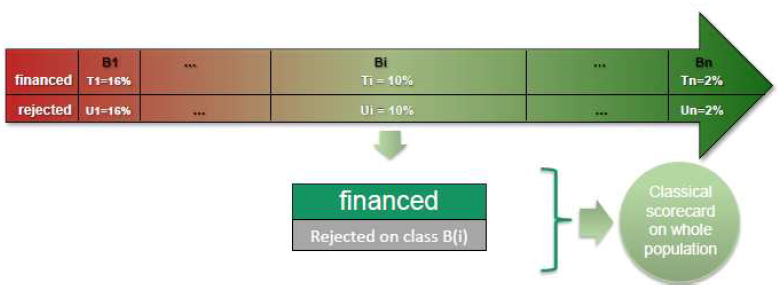
\includegraphics[width=0.5\textwidth]{figures/appendix/processusParcelling.png}
\caption{The accompanying Figure of the Parceling method in the internal documentation.}
\label{fig:parceling}
\end{figure}


\begin{table}
\caption{\label{parcel} Example of implementation of the Parcelling method on a small dataset}
{\setlength{\parindent}{0cm}
\begin{multicols}{3}

\begin{subfigure}[t]{0.31\textwidth}
\begin{center}
\begin{adjustbox}{max width=\textwidth}
\begin{tabular}{l l l}
\toprule
\textbf{Weight} & \textbf{${\bm{y}}_{\text{f}}$} & \textbf{${\bm{x}}_{\text{f}}$}\\
\midrule
1 & 1 & 0.562 \\
1 & 1 & 0.910 \\
1 & 0 & 0.430 \\
\bottomrule
\end{tabular}
\end{adjustbox}
\end{center}

\caption{Development of scorecard $p_{\hat{\gls{bth}}_\f}(1 | \gls{bx})$ on financed clients}
\label{parcel:sfig1}
\end{subfigure}

\columnbreak

\begin{subfigure}[t]{0.31\textwidth}
\begin{center}
\begin{adjustbox}{max width=\textwidth}
\begin{tabular}{l l l}
\toprule
\textbf{Score-band} & \textbf{$T$} &  \textbf{$U$} \\
\midrule
1 & 0.5 & 0.8 \\
... & ... & ... \\
K & 0.01 & 0.04 \\
\bottomrule
\end{tabular}
\end{adjustbox}
\end{center}

\caption{Calculation of $T(k)$ and $U(k)$}
\label{parcel:sfig2}
\end{subfigure}

\columnbreak

\begin{subfigure}[t]{0.31\textwidth}
\begin{center}
\begin{adjustbox}{max width=\textwidth}
\begin{tabular}{l l l}
\toprule
\textbf{Weight} & \textbf{${\bm{y}}$} & \textbf{${\bm{x}}$}\\
\midrule
1 & 0 & 0.562 \\
1 & 1 & 0.910 \\
1 & 0 & 0.430 \\
1 & 1 & 0.347 \\
1 & 0 & 0.140 \\
1 & 0 & 0.295 \\
\bottomrule
\end{tabular}
\end{adjustbox}
\end{center}

\caption{Inference for not financed clients}
\label{parcel:sfig3}
\end{subfigure}

\end{multicols}
}
\end{table}



\subsection{Simulation of reject inference methods applied to multivariate gaussian data} \label{subsec:app_reject_sim}

This early work aimed at comparing several reject inference methods in the well-specified model-case for 4 multivariate Gaussian features on Figure~\ref{fig:simu_4var} and 30 features on Figure~\ref{fig:simu_30var} in terms of error rate. The horizontal axis represents the cut-off value of a \gls{lr} that simulates the acceptance / rejection mechanism $p_{\gls{phi}}(\gls{z} | \gls{bx})$, such that it roughly corresponds to the fraction of missing labels $\gls{bby}_{\nf}$. In this setting, the semi-supervised generative approach obviously yields better results since the data lies in its restricted hypothesis space and it is able to use the predictors with missing labels $\gls{bbx}_{\nf}$. As explained thoroughly in Chapter~\ref{chap2}, standard \gls{lr} and Augmentation perform similarly (since they are both well-specified models and we are in a \gls{mar} setting). Parcelling does not work well since it is designed for a \gls{mnar} setting. In presence of well-separated data, Reclassification works well with 30 features since the true decision boundary is ``sharp'' (see the very small error rate) such that $\argmax_y \hat{p}(y | \gls{bx}) \approx \max_y \hat{p}(y | \gls{bx})$, which is less apparent with 4 features.


\begin{figure}[H]
\centering
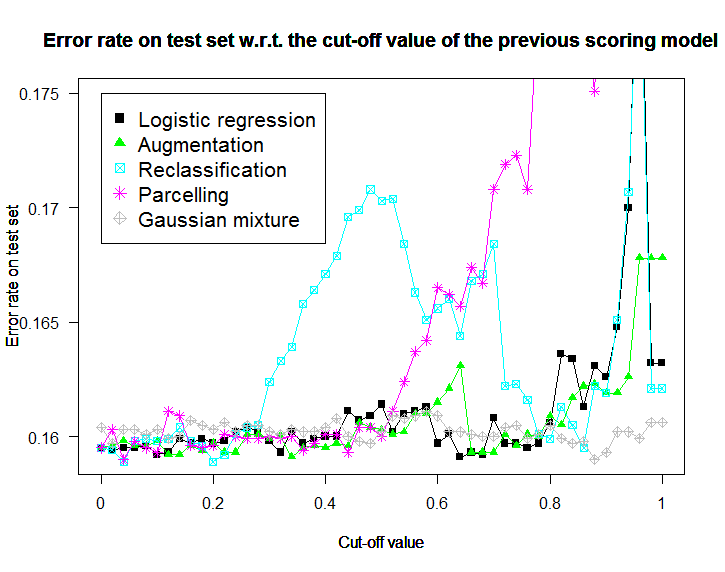
\includegraphics[width=0.4\textwidth]{figures/appendix/rejectinferencesimulation4var.png}
\caption{Simulation of multivariate 4-dimensional Gaussian features and performance of various reject inference methods including the proposed generative approach.}
\label{fig:simu_4var}
\end{figure}

\begin{figure}[H]
\centering
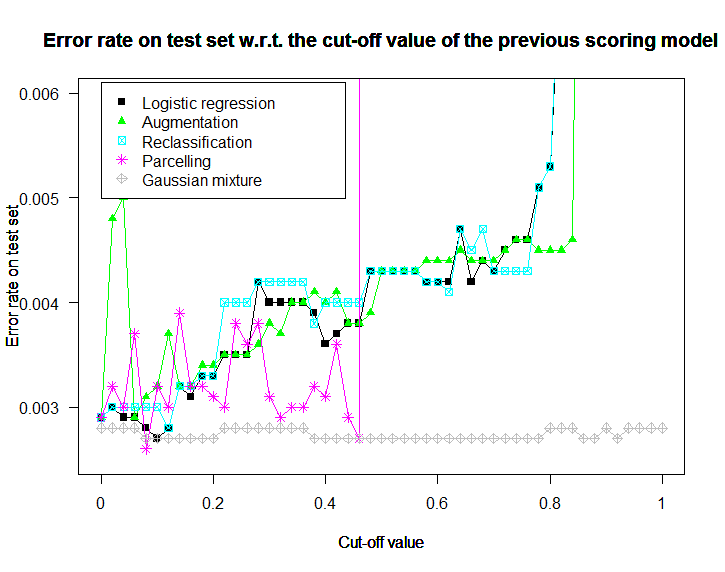
\includegraphics[width=0.4\textwidth]{figures/appendix/rejectinferencesimulation30var.png}
\caption{Simulation of multivariate 30-dimensional Gaussian features and performance of various reject inference methods including the proposed generative approach.}
\label{fig:simu_30var}
\end{figure}


%\subsection{Reject inference methods applied to real data: previous experiments} \label{subsec:app_reject_real}
%
%This early work shows all reject inference methods based on \gls{lr} applied to various \gls{cacf} datasets: Electronics loans, Sports goods and Standard loans in Figure~\ref{fig:darty_reject},~\ref{fig:decathlon_reject} and~\ref{fig:M3_reject} respectively (beware: the colors / symbols do not correspond to the same methods in each graph). The acceptance / rejection mechanism $p_{\gls{phi}}(\gls{z} | \gls{bx})$ is again simulated using a \gls{lr}. Two things are striking in these figures: first, all methods perform relatively similarly and suffer a big performance drop once the acceptance rate is below 50 \% (at which point there are very few ``bad borrower'' events - $y = 0$); second, the multivariate generative model that performed best on simulated data in the previous section performs worst with real data, since it makes more hypotheses and is thus less flexible.
%
%\begin{figure}[H]
%\centering
%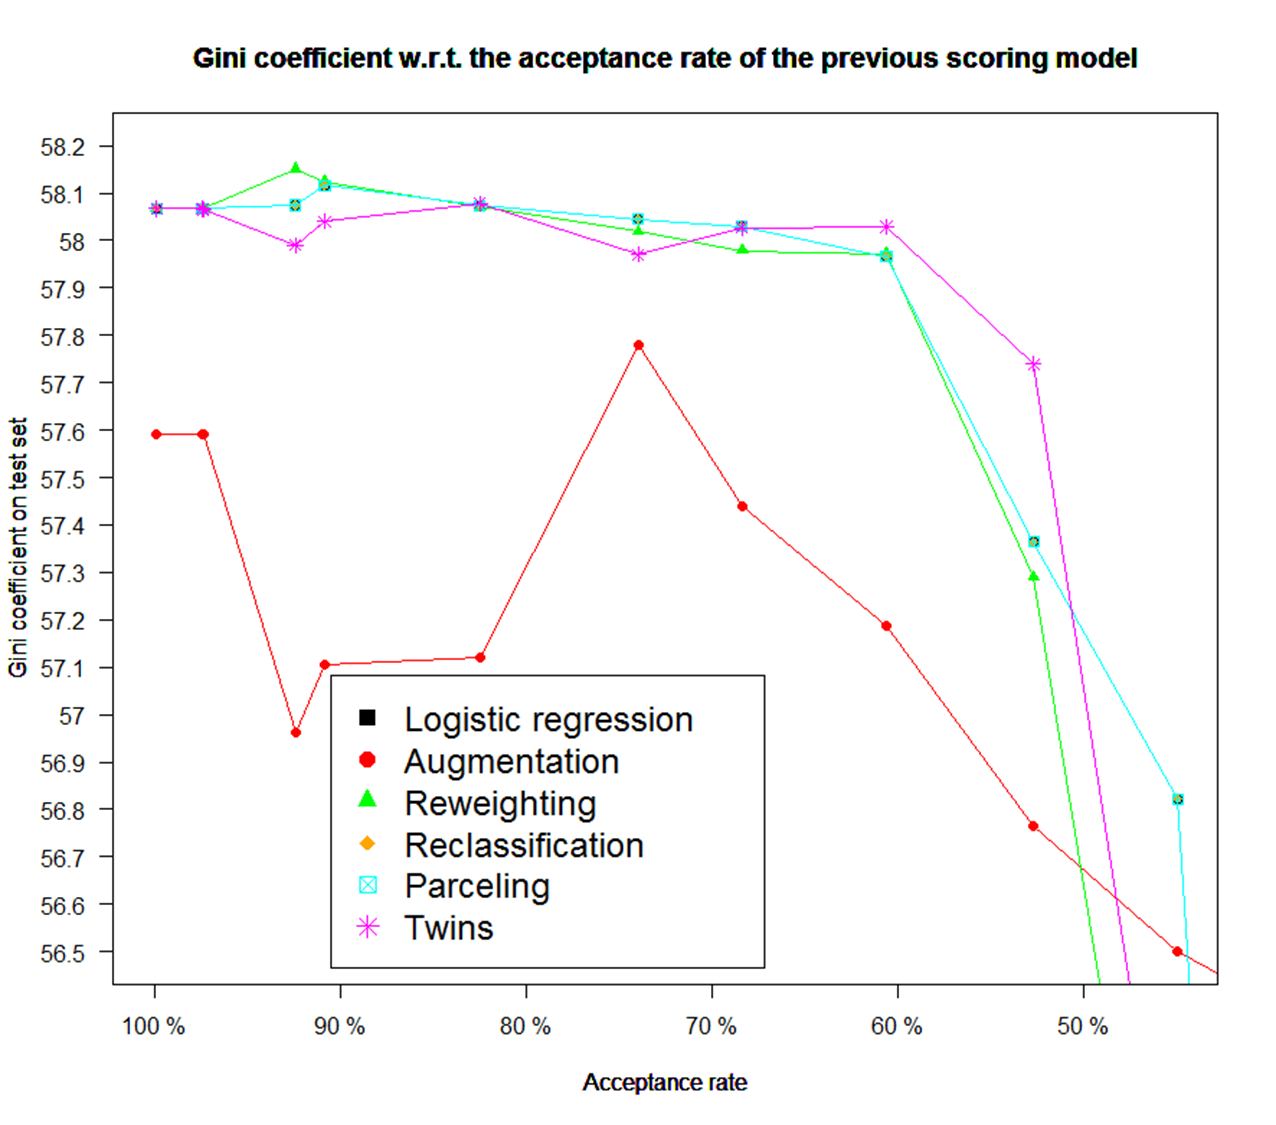
\includegraphics[width=0.4\textwidth]{figures/appendix/rejectinferencedarty3.png}
%\caption{Performance resulting from the use of reject inference methods in terms of Gini on an Electronics loans dataset from \gls{cacf}.}
%\label{fig:darty_reject}
%\end{figure}
%
%\begin{figure}[H]
%\centering
%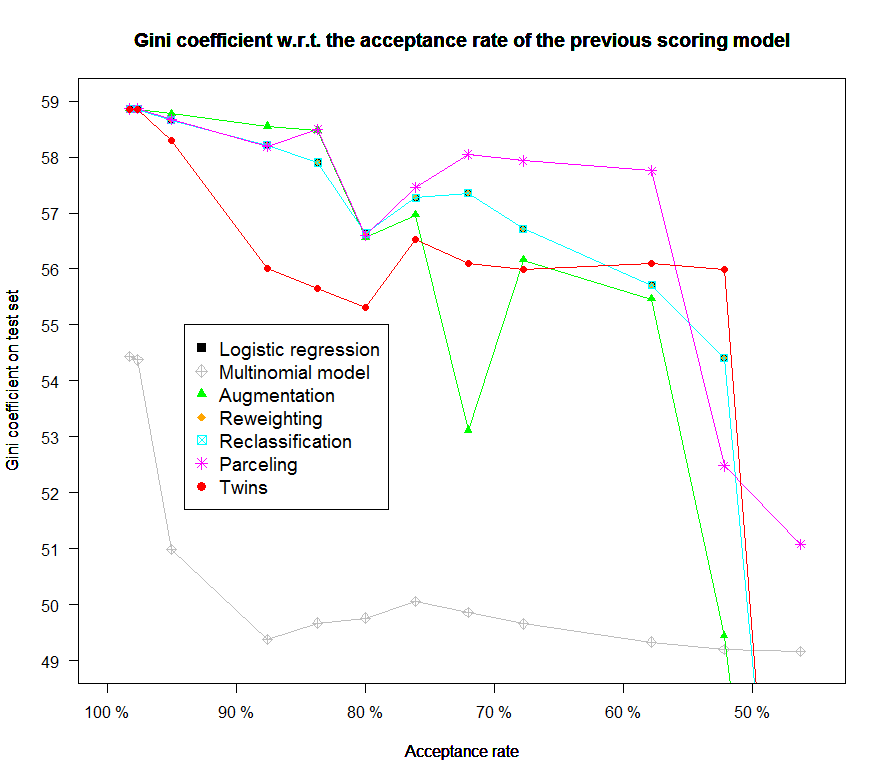
\includegraphics[width=0.4\textwidth]{figures/appendix/rejectinferencedecathlon.png}
%\caption{Performance resulting from the use of reject inference methods in terms of Gini on a Sports goods loans dataset from \gls{cacf}.}
%\label{fig:decathlon_reject}
%\end{figure}
%
%\begin{figure}[H]
%\centering
%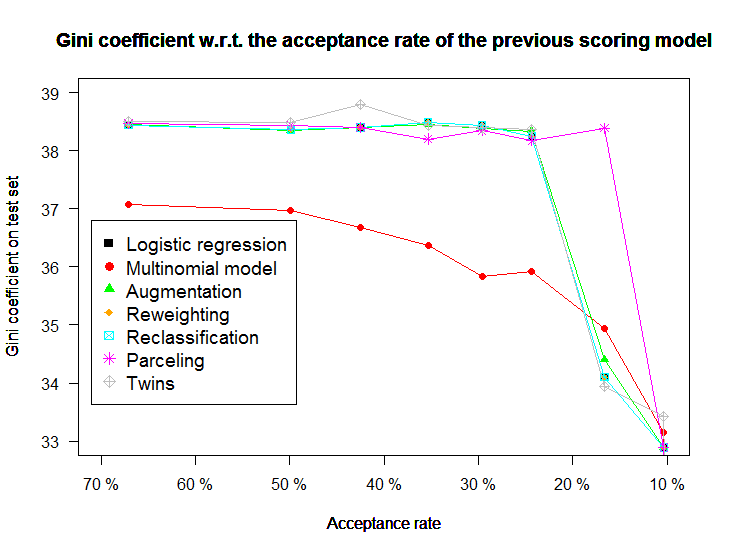
\includegraphics[width=0.4\textwidth]{figures/appendix/rejectinferenceM3.png}
%\caption{Performance resulting from the use of Reject Inference methods in terms of Gini on a Standard loans dataset from \gls{cacf}.}
%\label{fig:M3_reject}
%\end{figure}


\subsection{Performance of other predictive models w.r.t.\ the acceptance level} \label{subsec:app_reject_real_method}

Also part of an earlier work, this section's aim was to compare the performance of other ``machine learning'' models than simple \gls{lr} (although we purposely restricted our focus in Chapter~\ref{chap2} to the \gls{lr}) to see if, when presented with the same data and in presence of a simulated acceptance / rejection mechanism as earlier showcased, it would not be of better interest to switch to a different model, although it was argued in Chapter~\ref{chap2} that these models would not perform good under a \gls{mar} setting. The same datasets as in the previous section are used: the proposed models all perform poorer than \gls{lr} but most importantly their performance drops significantly with the proportion of simulated accepted clients.

\begin{figure}[H]
\centering
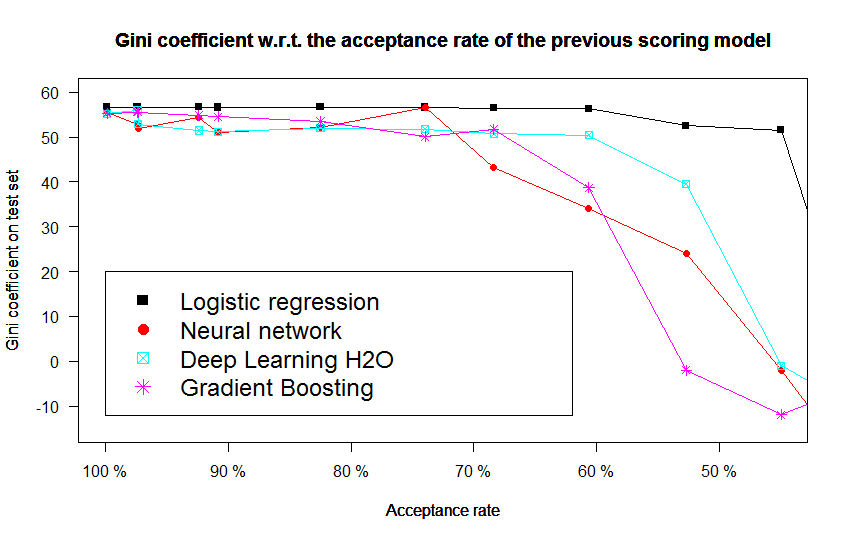
\includegraphics[width=0.4\textwidth]{figures/appendix/newmodelsdarty.png}
\caption{Performance resulting from the use of other predictive methods in terms of Gini on an Electronics loans dataset from \gls{cacf}.}
\label{fig:darty_othermodels}
\end{figure}

\begin{figure}[H]
\centering
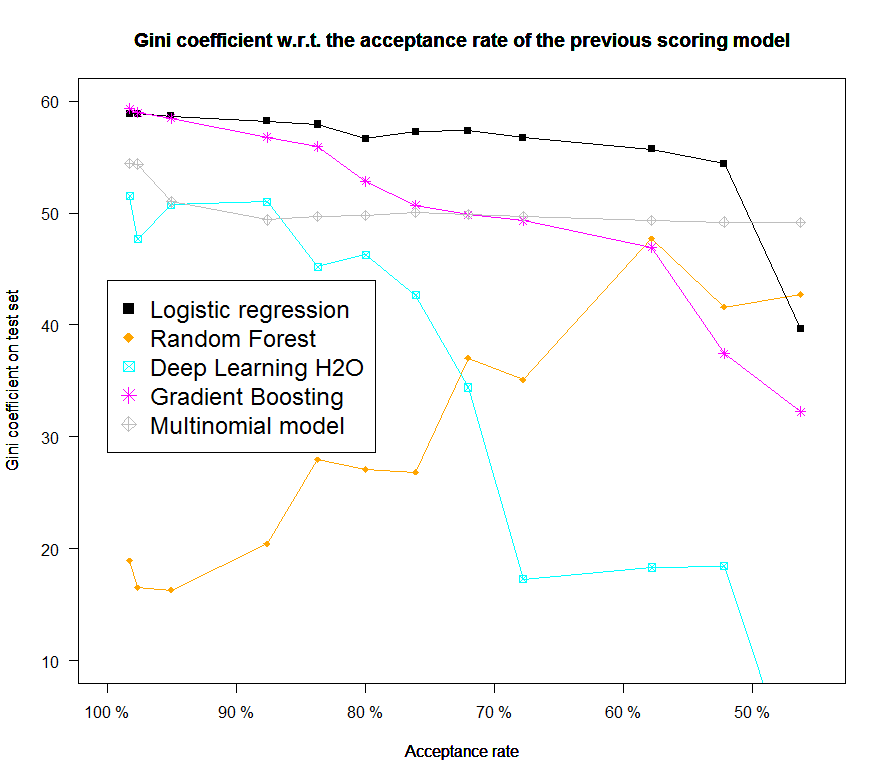
\includegraphics[width=0.4\textwidth]{figures/appendix/newmodelsdecathlon.png}
\caption{Performance resulting from the use of other predictive methods in terms of Gini on a Sports good loans dataset from \gls{cacf}.}
\label{fig:decathlon_othermodels}
\end{figure}

\begin{figure}[H]
\centering
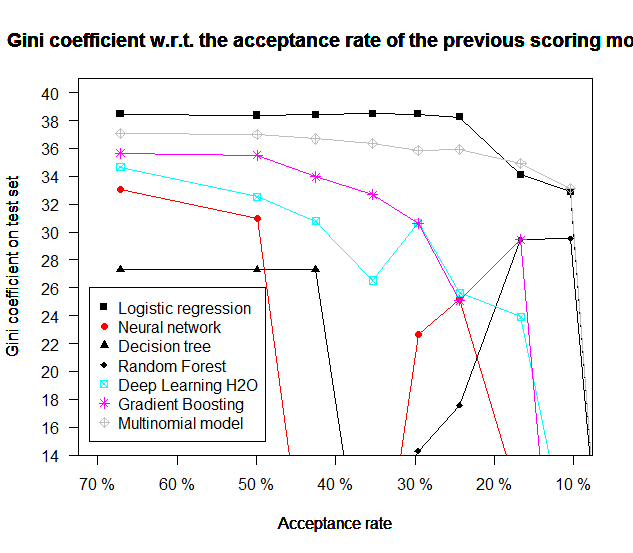
\includegraphics[width=0.4\textwidth]{figures/appendix/newmodelsm3web.png}
\caption{Performance resulting from the use of other predictive methods in terms of Gini on a Standard loans dataset from \gls{cacf}.}
\label{fig:M3_othermodels}
\end{figure}


\section{Discretization methods}

\subsection{Unsupervised methods}

\subsubsection{The \textit{equal-freq} algorithm}

The \textit{equal-freq} algorithm~\ref{equal-freq-disc} is illustrated on Figure~\ref{fig:disc_equal_freq}. 

\begin{figure}[H]
\centering
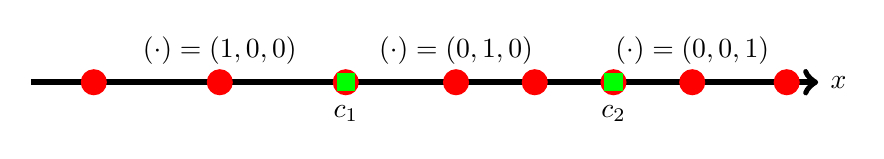
\begin{tikzpicture}[scale=0.2,every node/.style={scale=1}]
\draw[->,line width=0.08cm] (-12,0)--(38,0) node[right]{$\gls{x}$};

% Original data points
\node [red,circle, fill] at (-8,0) {};
\node [red,circle, fill] at (0,0) {};
\node [red,circle, fill] at (8,0) {};
\node [red,circle, fill] at (15,0) {};
\node [red,circle, fill] at (20,0) {};
\node [red,circle, fill] at (25,0) {};
\node [red,circle, fill] at (30,0) {};
\node [red,circle, fill] at (36,0) {};


% Cut points
\node [green,rectangle,rotate=90,fill] at (8,0) {};
\node [green,rectangle,rotate=90,fill] at (25,0) {};

\node at (8,-2) {$c_1$};
\node at (25,-2) {$c_2$};

% Disc value
\node at (0,2) {$\q(\cdot) = (1,0,0)$};
\node at (15,2) {$\q(\cdot) = (0,1,0)$};
\node at (30,2) {$\q(\cdot) = (0,0,1)$};


\end{tikzpicture}
\caption{\label{fig:disc_equal_freq} Original data in \textcolor{red}{red} is discretized using an \textit{equal-freq} procedure resulting in $m=3$ intervals using the two cutpoints in \textcolor{green}{green}.}
\end{figure}



\begin{algorithm}[H]
 \KwData{$n,\gls{bbx},(m_j)_1^d$}
 \KwResult{$\hat{\q}$}
 \For{$j=1$ to $d$}{
Sort $\gls{bbx}^j$ by ascending order\;
Let $c_0=-\infty$, $c_{m_j} = + \infty$ and $c_{j,h} = x_{\left\lceil{{\frac{h \cdot n}{m_j}}}\right\rceil,j}$\;
Let $C_{j,h} = ]c_{j,h-1};c_{j,h}]$ and $\hat{\q}_j(\cdot) = (\hat{q}_{j,h}(\cdot))_1^{m_j}$\;
Set $\hat{q}_{j,h}(\cdot)=\mathds{1}_{C_{j,h}}(\cdot)$.
%\For{$i=1$ to $n$}{
%Set $q_i^j(x_j) = \begin{cases} 1 \text{ si } x_i^j \leq x_{\left\lceil{{\frac{n}{m_j}}}\right\rceil}^j \\ o \text{ si } x_{\left\lceil{{\frac{(o-1)*n}{m_j}}}\right\rceil}^j < x_i^j \leq x_{\left\lceil{{\frac{o*n}{m_j}}}\right\rceil}^j \\ m_j \text{ si } x_{\left\lceil{{\frac{(m_j-1)*n}{m_j}}}\right\rceil}^j < x_i^j \end{cases}$
%}
}
 \caption{\label{equal-freq-disc} \textit{equal-freq} discretization: an equal number of training observations are in each bin.}
\end{algorithm}


\subsubsection{The \textit{equal-length} algorithm} \label{app1:equal_length}

The \textit{equal-length} algorithm~\ref{equal-length-disc} is illustrated on Figure~\ref{fig:disc_equal_length}. 

\begin{figure}[H]
\centering
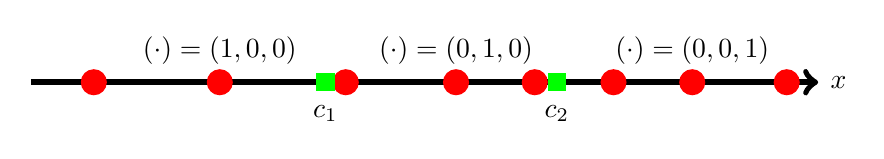
\begin{tikzpicture}[scale=0.2,every node/.style={scale=1}]
\draw[->,line width=0.08cm] (-12,0)--(38,0) node[right]{$\gls{x}$};

% Original data points
\node [red,circle, fill] at (-8,0) {};
\node [red,circle, fill] at (0,0) {};
\node [red,circle, fill] at (8,0) {};
\node [red,circle, fill] at (15,0) {};
\node [red,circle, fill] at (20,0) {};
\node [red,circle, fill] at (25,0) {};
\node [red,circle, fill] at (30,0) {};
\node [red,circle, fill] at (36,0) {};


% Cut points
\node [green,rectangle,rotate=90,fill] at (6.7,0) {};
\node [green,rectangle,rotate=90,fill] at (21.4,0) {};

\node at (6.7,-2) {$c_1$};
\node at (21.4,-2) {$c_2$};

% Disc value
\node at (0,2) {$\q(\cdot) = (1,0,0)$};
\node at (15,2) {$\q(\cdot) = (0,1,0)$};
\node at (30,2) {$\q(\cdot) = (0,0,1)$};


\end{tikzpicture}
\caption{\label{fig:disc_equal_length} Original data in \textcolor{red}{red} is discretized using an \textit{equal-length} procedure resulting in $m=3$ intervals using the two cutpoints in \textcolor{green}{green}.}
\end{figure}


\begin{algorithm}[H]
 \KwData{$n,\gls{bbx},(m_j)_1^d$}
 \KwResult{$\hat{\q}$}
 \For{$j=1$ to $d$}{
Let $w_j = \max_{i} x_{i,j} - \min_{i} x_{i,j}$\;
Let $c_0=-\infty$, $c_{m_j} = + \infty$ and $c_{j,h} = \frac{w_j \cdot h}{m_j} + \min_{i} x_{i,j}$\;
Let $C_{j,h} = ]c_{j,h-1};c_{j,h}]$ and $\hat{\q}_j(\cdot) = (\hat{q}_{j,h}(\cdot))_1^{m_j}$\;
Set $\hat{q}_{j,h}(\cdot)=\mathds{1}_{C_{j,h}}(\cdot)$.
}
 \caption{\label{equal-length-disc} \textit{equal-length} discretization: each bin has the width of the training set's total support divided by the number of bins.}
\end{algorithm}



\subsection{Supervised univariate methods}

\subsubsection{The \textit{ChiMerge} algorithm}

\textit{ChiMerge}~\cite{kerber1992chimerge}, given in Algorithm~\ref{chimerge}, is a supervised (it takes into account the labels $\gls{bby}$) univariate (it does not take into account the other features $\gls{bbx}_{\{-j\}}$)). It is used indirectly in the benchmarks of Chapter~\ref{chap4} where we applied the same approach to categorical features by computing all the pairwise $\chi^2$ indepedence tests. Here we showcase a rather na\"{\i}ve implementation as a pseudo-code in Algorithm~\ref{chicollapse}, which in practice would perform poorly (because of exponential complexity in the number of categories $l_j$) but, from an iteration to another, a lot of $\chi^2$ tests are unaffected, so they can be stored rather than computed again. The initial and final steps of \textit{ChiMerge} are illustrated in Table~\ref{tab:chimerge_ex}. Refinements of the method, taking into account multiple testing and / or adapting the tests' siognificance level $\alpha$ to each feature, were done in~\cite{liu1995chi2,wang1998concurrent,tay2002modified,su2005extended}.

%\begin{table}
%\centering
%\caption{\label{tab:chimerge_ex} p-values of $\chi^2$ tests between subsequent categories. The pair of categories the least independent (\textit{i.e.}\ with highest p-value) is $(-\infty-18,18-20)$ which should be merged into $-\infty-20$.}
%\begin{tabular}{p{2.5cm}|p{2.5cm}|p{2.5cm}|p{2.5cm}}
%Category & \# samples & \# $\{Y=1\}$ & p-value \\
%\hline
%$-\infty$-18 & 10 & 5 & \multirow{2}{*}{\textbf{1}} \\
%18-20 & 10 & 5 & \multirow{2}{*}{0.3} \\
%20-22 & 10 & 6 & \multirow{2}{*}{0.2} \\
%22-24 & 10 & 4 & \multirow{2}{*}{0.2}\\
%24-$+\infty$ & 10 & 2 & \multirow{2}{*}{0.2} \\
%\dots & \dots & \dots & \dots \\
%\end{tabular}
%\end{table}
%
%\textcolor{red}{calculer les chi 2 exacts}

\begin{table}
\caption{\label{tab:chimerge_ex} p-values of $\chi^2$ tests between subsequent categories on the iris dataset.}
\centering
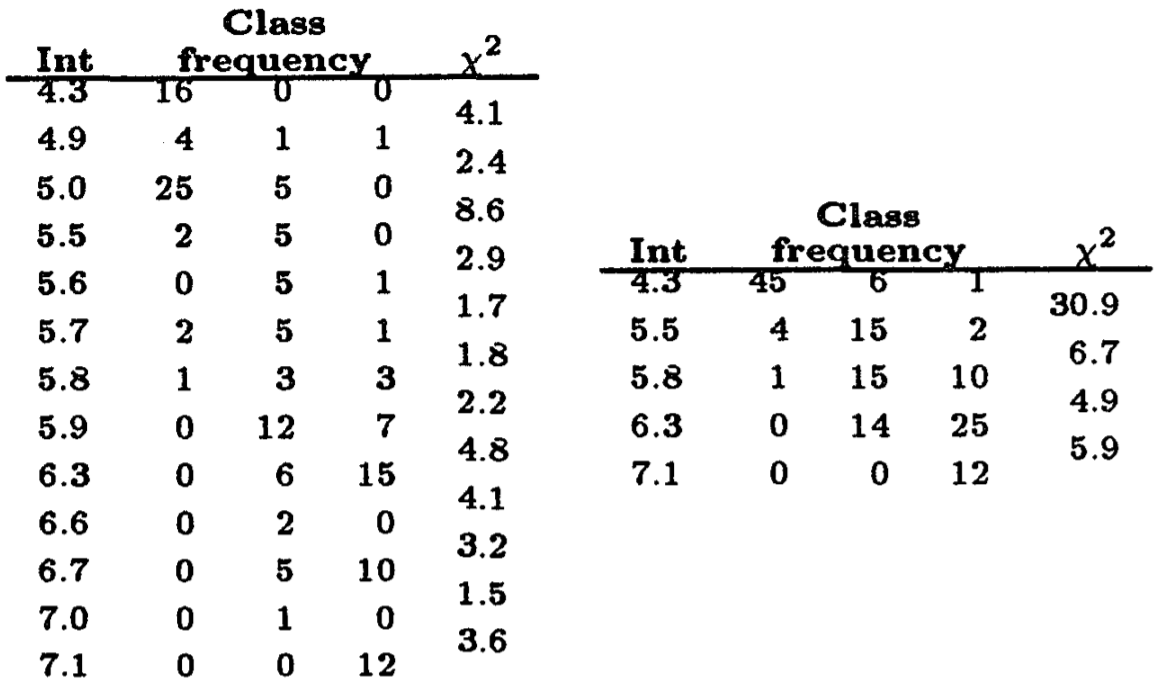
\includegraphics[width = .7\textwidth]{figures/appendix/tab_chimerge.PNG}
\end{table}

\begin{algorithm}[H]
 \KwData{$n,\gls{bbx},\alpha$}
 \KwResult{$\hat{\q}$}
 \For{$j=1$ to $d$}{
 $\alpha_{\text{max}}$ = 1\;
 Sort $\gls{bbx}_j$ in ascending order\;
 Let $c_0=-\infty$, $m_j = n$, $c_{m_j} = + \infty$ and $c_{j,h} = \frac{x_{i,j} + x_{i+1,j}}{2}$ for $1 \leq i \leq n-1$\;
 \While{$\alpha_{\text{max}} > \alpha$}{
Let $C_{j,h} = ]c_{j,h-1};c_{j,h}]$ and $\hat{\q}_j(\cdot) = (\hat{q}_{j,h}(\cdot))_1^{m_j}$\;
Set $\hat{q}_{j,h}(\cdot)=\mathds{1}_{C_{j,h}}(\cdot)$\;
%Perform $\chi^2$ tests of independence among all contiguous pairs\:
\For{$1 \leq h \leq m_j-1$}{
$\chi^2_h = \sum_{h'=h}^{h+1} \sum_{y=0}^{1} \frac{ \left( \sum_{i=1}^n \mathds{1}_{y}(y_i) \hat{q}_{j,h'}(x_{i,j} ) - \frac{\sum_{i=1}^n \hat{q}_{j,h'}(x_{i,j}) \times \sum_{i=1}^n \mathds{1}_{y}(y_i)}{n} \right)^2}{\frac{\sum_{i=1}^n \hat{q}_{j,h'}(x_{i,j}) \times \sum_{i=1}^n \mathds{1}_{y}(y_i)}{n}}$\;
}
%Under the null hypothesis that two consecutive intervals are independent w.r.t.\ the target $y$, $\chi^2_h$ is $\chi^2$-distributed (1 degree of freedom)\;
Let $c_{j,\argmin_h \chi^2_h} = \frac{c_{j,h} + c_{j,h+1}}{2}$ and $c_{j,h'} \leftarrow c_{j,h'+1}$ for $\argmin_h \chi^2_h < h' < m_j$\;
Let $m_j \leftarrow m_j-1$\;
Let $X \sim \chi^2$ and $\alpha_{\max} = \max_h p(X \geq \chi^2_h) = p(X \geq \min_h \chi^2_h)$.
}
}
 \caption{\label{chimerge} The ChiMerge algorithm discretizes features by performing $\chi^2$ tests recursively at a user-defined level $\alpha$.}
\end{algorithm}


\subsubsection{The \textit{MDLP} algorithm} \label{app1:mdlp}

The \textit{MDLP} algorithm~\cite{fayyad1993multi} is an entropy-based discretization method. Contrary to ChiMerge, where at the beginning all distinct values are put into separate categories and thereafter merged (bottom-up method), MDLP recursively calculates the entropy produced by each candidate cutpoint on their subsequent binary splits. It is reproduced in Algorithm~\ref{mdlp}.

\begin{algorithm}[H]
 \KwData{A continuous feature $\gls{bbx}_j$ which subscript $j$ is dropped in what follows; targets $\gls{bby}$.}
 \KwResult{Cutpoints $\mathcal{C}_\star$}
 Initialize $\mathcal{C}_\star = \varnothing$\;
Order $\gls{bbx}$\;
Compute the set $\mathcal{I}$ of indices $i$ such that $y_i \neq y_{i+1}$ (contiguous observations which are not of the same class)\;
Compute the set of candidate cutpoints $\mathcal{C}$ as the mean between these points, \textit{i.e.}\ $\mathcal{C} = \{\frac{x_i + x_{i+1}}{2} | i \in \mathcal{I} \}$\;
Compute the class entropy of each candidate cutpoint $c \in \mathcal{C}$ as:
\[ \text{E}(c) = \frac{|\gls{bbx} < c|}{|\gls{bbx}|} \text{Ent}(\gls{bbx} < c) + \frac{|\gls{bbx} > c|}{|\gls{bbx}|} \text{Ent}(\gls{bbx} > c), \]
where $\text{Ent}(\gls{bbx} < c) = - \sum_{y=0}^1 p(y,\gls{bbx} < c) \ln p(y,\gls{bbx} < c)$ and $p$ is estimated \textit{via} class proportions, \textit{i.e.}\ $p(y,\gls{bbx} < c) = \frac{|\{i | y_i = y \& x_i < c \}|}{|\gls{bbx} < c|}$\;
Select $c_\star$ which minimizes $\text{E}(c)$ and append it to $\mathcal{C}_\star$\;
Repeat steps for $\{\gls{bbx}< c\}$ and $\{\gls{bbx} > c\}$\;
Stop when $\text{Gain}(c,\gls{bbx}) = \text{E}(c) - \text{Ent}(\gls{bbx}) \leq \frac{\ln_2 (|\gls{bbx}|-1)}{|\gls{bbx}|} + \frac{\Delta(c,\gls{bbx}) }{|\gls{bbx}|}$ where $\Delta(c,\gls{bbx}) = \ln_2 7 - (k \text{Ent}(\gls{bbx}) - k_{<c}\text{Ent}(\gls{bbx} < c) - k_{>c}\text{Ent}(\gls{bbx} < c))$ and $k$, $k_{<c}$, $k_{>c}$ represent the number of classes (1 or 2 in the binary setting) in their respective sample $\gls{bbx}$, $\gls{bbx} < c$ and $\gls{bbx} > c$\;
 \caption{\label{mdlp} The MDLP algorithm recursively performs discretization with an information gain criterion.}
\end{algorithm}


\subsection{Proposal: \textit{glmdisc}}


\subsubsection{\textit{glmdisc} with neural networks} \label{app1:glmdiscNN}

This section describes the \textit{glmdisc}-NN algorithm developed in Chapter~\ref{chap4} and examplifies it on simulated data in Figure~\ref{fig:animNN}.

\begin{algorithm}[H]
 \KwData{$((\gls{bbx}_j)_1^{d}, \gls{bby}),S,\bm{m}_\text{start}$}
 \KwResult{$\hat{\q}^{(s_\star)}$}
 Initialization of the network: for each feature feature $j$, add a softmax with $m_{j,\text{start}}$ outputs which are themselves combined in a sigmoid neuron\;
 Initialization of the network's weights at random\;
 $s = 0$\;
 \While{$s < S$}{
Perform feed-forward pass of the data: calculate $p_{\gls{bth}^{(s)}}(\gls{bby} | \q_{\ag^{(s)}}(\gls{bbx}))$\;
Perform back-propagation of the error via Stochastic Gradient Descent which yields parameters $(\gls{bth}^{(s+1)},\ag^{(s+1)})$\;
 Compute the \textit{maximum a posteriori} of the hidden layer's representations $\hat{\q}^{(s)}(\gls{bbx})$ such that $\hat{q}_{j,h}(x_j) = 1 \text{ if } h = \argmax_{1 \leq h' \leq m_j} q_{\hat{\ag}_{j,h'}}, 0 \text{ otherwise.}$\;
 Compute the associated \gls{lr} parameters $\hat{\gls{bth}}^{(s)} = \argmax_{\gls{bth}} \ell(\gls{bth} ; {\hat{\q}_j^{(s)}}, \gls{bby})$\;
    $s \leftarrow s+1$\;
}
 Choose the best quantization $\hat{\q}^{(s_\star)}$, which associated \gls{lr} parameters yield the lowest BIC criterion\;
 \caption{\label{NN-disc} \textit{glmdisc}-NN: supervised multivariate quantization for logistic regression with neural networks.}
\end{algorithm}

\begin{figure}[!h]
\begin{animateinline}[poster=first, controls=all, palindrome, autopause, autoresume, width=\textwidth, height=6cm]{3}
\multiframe{200}{i=1+1}{\input{R_CODE_FIGURES/appendix/animation_disc_tensorflow/False_simulated_data/feature_0_iteration_\i.tex}}%
\end{animateinline}
\caption{\label{fig:animNN} Animation of the softmax activation functions $\q_{\ag^{(s)}}$ over the epoch $(s)$.}
\end{figure}


%\textcolor{red}{à décommenter // ajouter caption}

\subsubsection{\textit{glmdisc} with an \gls{sem} algorithm} \label{app1:glmdiscSEM}

This section describes the \textit{glmdisc}-SEM algorithm developed in Chapter~\ref{chap4} and examplifies it on simulated data in Figure~\ref{fig:animSEM}.

\begin{algorithm}[H]
 \KwData{$((\gls{bbx}_j)_1^{d}, \gls{bby}),S,\bm{m}_\text{start}$}
 \KwResult{$\hat{\bbqk}^{(s_\star)}$}
 Initialization of $\bbqk_j^{(0)}$ at random in $\{1, \dots, m_{j,\text{start}}\}$ and one-hot encode the resulting vector\;
 $s = 0$\;
 \While{$s < S$}{
  Adjust logistic regression $\gls{bth}^{(s)} = \argmax_{\gls{bth}} \ell(\gls{bth};\bbqk^{(s)}, \gls{bby})$\;
  \For{$j = 1$ \KwTo $d$}{
   Adjust multinomial logistic regression or contingency tables $\ag_j^{(s)} = \argmax_{\ag_j} \ell(\ag_j;\gls{bbx}_j,\bbqk_j^{(s)})$\;
Draw new latent features ${\bqk_j^{(s+1)}} \sim \text{ Mult} \left( p_{\gls{bth}^{(s)}}(y | \bqk^{(s)}_{-\{ j \}}, \cdot) p_{\ag_j^{(s)}}(\cdot | \gls{bx}_j) \right)$ for each observation (the subscript $i$ is voluntarily omitted)\;
 Compute the \textit{maximum a posteriori} of these latent features for all observations ${\hat{\bqk}_j^{(s)}} = \argmax_{\bqk_j} p_{\ag_j^{(s)}}(\bqk_j | \gls{bx}_j)$\;
 Compute the associated \gls{lr} parameters $\hat{\gls{bth}}^{(s)} = \argmax_{\gls{bth}} \ell(\gls{bth} ; {\hat{\bbqk}_j^{(s)}}, \gls{bby})$\;
   }
   $s \leftarrow s+1$\;
 }
 Choose the best quantization $\hat{\bbqk}^{(s_\star)}$, which associated \gls{lr} parameters $\hat{\gls{bth}}^{(s_\star)}$ yield the lowest BIC criterion.
 \caption{\label{SEM-disc} \textit{glmdisc}-SEM: supervised multivariate quantization for logistic regression with an \gls{sem} algorithm.}
\end{algorithm}

\begin{figure}[!h]
\begin{animateinline}[poster=first, controls=all, palindrome, autopause, autoresume, width=\textwidth, height=10cm]{5}
\multiframe{200}{i=1+1}{\input{R_CODE_FIGURES/appendix/animation_disc_SEM/sem_simulated_data/sem_feature_1_iter_\i.tex}}%
\end{animateinline}
\caption{\label{fig:animSEM} Animation of the $\bqk_j$ of \textit{glmdisc}-SEM through the iterations $(s)$.}
\end{figure}

%\textcolor{red}{à décommenter // ajouter caption  et numéro itération}


\section{Factor levels grouping method} \label{app1:chicollapse}

As part of Chapter~\ref{chap4}, we gave results for competing methods MDLP / $\chi^2$ tests where the $\chi^2$ tests can be explicited in Algorithm~\ref{chicollapse} which I called ChiCollapse. My rather na{\"\i}ve implementation (where, as in the pseudo-code, all pairwise $\chi^2$ tests are recalculated at each step) is available as a gist on Github at \url{https://gist.github.com/adimajo/eb007492007d650091f6bd7cb2047493}. An example of the resulting usage of the grouped levels in a predictive setting is also given as a gist on Github at \url{https://gist.github.com/adimajo/8f8401b59ba838c65534673842b0f60d}.

\begin{algorithm}[H]
 \KwData{$n,\gls{bbx},\alpha$}
 \KwResult{$\hat{\q}$}
 \For{$j=1$ to $d$}{
 $\alpha_{\text{max}}$ = 1\;
 Let $C_{j,h} = \{h\}$ for $1 \leq i \leq l_j$\;
 \While{$\alpha_{\text{max}} > \alpha$}{
Let $\hat{\q}_j(\cdot) = (\hat{q}_{j,h}(\cdot))_1^{m_j}$\;
Set $\hat{q}_{j,h}(\cdot)=\mathds{1}_{C_{j,h}}(\cdot)$\;
%Perform all pairwise $\chi^2$ tests of independence among all contiguous pairs\:
\For{$1 \leq h_1 < h_2 \leq m_j$}{
$\chi^2_{h_1,h_2} = \sum_{h'=h_1}^{h_2} \sum_{y=0}^{1} \frac{ \left( \sum_{i=1}^n \mathds{1}_{y}(y_i) \hat{q}_{j,h'}(x_{i,j} ) - \frac{\sum_{i=1}^n \hat{q}_{j,h'}(x_{i,j}) \times \sum_{i=1}^n \mathds{1}_{y}(y_i)}{n} \right)^2}{\frac{\sum_{i=1}^n \hat{q}_{j,h'}(x_{i,j}) \times \sum_{i=1}^n \mathds{1}_{y}(y_i)}{n}}$\;}
%Under the null hypothesis that two factor levels are independent w.r.t.\ the target $y$, $\chi^2_{h_1,h_2}$ is $\chi^2$-distributed (1 degree of freedom)\;
Let $(h_1,h_2) = \argmin_{h_1,h_2} \chi^2_{h_1,h_2}$, $C_{j,h_1} = C_{j,h_1} \cup C_{j,h_2}$ and $C_{j,h} \leftarrow C_{j,h+1}$ for $h_2 \leq h < m_j$\;
Let $m_j \leftarrow m_j-1$\;
Let $X \sim \chi^2$ and $\alpha_{\max} = \max_{h_1,h_2} p(X \geq \chi^2_{h_1,h_2}) = p(X \geq \min_{h_1,h_2} \chi^2_{h_1,h_2})$.
}
}
 \caption{\label{chicollapse} ChiCollapse algorithm: adaptation of ChiMerge to categorical features.}
\end{algorithm}


%\section{Interaction discovery methods}



\section{Logistic regression-based trees}


%\subsection{\gls{pca}} \label{app1:sec_pca}
%
%\begin{algorithm}[H]
% \KwData{$\gls{bbx}$}
% \KwResult{$\gls{bbx}$}
%
% \caption{\label{alg:pca} \gls{pca} algorithm.}
%\end{algorithm}

%\subsection{\gls{mca}} \label{app1:sec_mca}
%
%\begin{algorithm}[H]
% \KwData{$n,\gls{bbx},\alpha$}
% \KwResult{$\hat{\q}$}
%
% \caption{\label{alg:mca} \gls{mca} algorithm.}
%\end{algorithm}


%\subsection{\gls{famd}} \label{app1:sec_famd}
%
%\begin{algorithm}[H]
% \KwData{$n,\gls{bbx},\alpha$}
% \KwResult{$\hat{\q}$}
%
% \caption{\label{alg:famd} \gls{famd} algorithm.}
%\end{algorithm}


\subsection{LogitBoost} \label{LogitBoost}

The LogitBoost algorithm~\cite{friedman2000additive} for 2 classes is equivalent to the Iterative Reweighted Least Squares method~\cite{friedman2001elements}. However, in \gls{lmt}, in order to perform feature selection, a slight modification is brought to the algorithm so as to fit univariate regressions and pick the best. It is given in Algorithm~\ref{alg:logitboost}.

\begin{algorithm}[H]
 \KwData{$n,\gls{bbx},\gls{bby}, S$}
 \KwResult{$F(\gls{bx})$}
Let weights $w_i = 1 / n$, $F(x) = 0$, $p(1 | \gls{bx}) = \frac{\exp(F(\gls{bx})}{\exp(F(\gls{bx}) + \exp(-F(\gls{bx})}$\;
\For{$s = 1$ to $S$}{
Compute weights $\mathbf{w} = p(1 | \gls{bbx}) \odot (\mathbf{1} - p(1 | \gls{bbx}))$\;
Compute response $z_{i} = \frac{y_i - p(1 | \gls{bx})}{w_i}$\;
\For{$j = 1$ to $d$}{
Fit the univariate reweighted regression coefficient $\hat{\theta}_{s,j} = \argmin_\theta \sum_{i=1}^n w_i \cdot (z_i - \theta x_{i,j})^2 $\;
}
Retrieve the best univariate coefficient $j^{\star} = \argmin_{1 \leq j \leq d} \sum_{i=1}^n w_i \cdot (z_i - \hat{\theta}_{s,j} x_{i,j})^2 $\;
Update $F(\gls{bx}) = F(\gls{bx}) + \frac{1}{2} \hat{\theta}_{s,j^\star} x_j$\;
}
 \caption{\label{alg:logitboost} LogitBoost algorithm.}
\end{algorithm}


\subsection{\gls{pls}} \label{app1:sec_pls}

The \gls{pls} algorithm given in~\eqref{alg:pls} has been proposed in~\cite{wold1984collinearity}. This version is adapted from~\cite{friedman2001elements} (Algorithm 3.3 in Section 3.5.2 p.\ 81).

\begin{algorithm}[H]
 \KwData{$\gls{bbx},\gls{bby}$}
 \KwResult{$\mathbf{z}$}
Standardize each $\gls{bbx}_j$ to have mean zero and variance one (which implies that categorical features have been one-hot encoded prior to this step) \;
Set $\hat{\gls{bby}}^{(0)} = |\gls{bby}| \mathbf{1}$\;
Set $\gls{bbx}_j^{(0)} = \gls{bbx}_j$\;
\For{$j=1$ to $d$}{
Let $\mathbf{z}_j = \sum_{j {'} = 1}^d \hat{\phi}_{j,j {'} } \gls{bbx}_{j {'} }^{(j-1)}$ where $\hat{\phi}_{j,j {'} } = \gls{bbx}_{j {'} }^{(j-1)} {'} \gls{bby}$ \;
Let $\theta_j = \frac{\mathbf{z}_j {'} \gls{bby}}{\mathbf{z}_j {'} \mathbf{z}_j}$\;
Let $\hat{\gls{bby}}^{(j)} = \hat{\gls{bby}}^{(j-1)} + \theta_j \mathbf{z}_j$\;
Orthogonalize each $\gls{bbx}_{j{'}}^{(j-1)}$ w.r.t.\ $\mathbf{z}_j$: $\gls{bbx}_{j{'}}^{(j)} = \gls{bbx}_{j{'}}^{(j-1)} - \frac{\mathbf{z}_j {'} \gls{bbx}_{j{'}}^{(j-1)}}{\mathbf{z}_{j} {'} \mathbf{z}_j} \mathbf{z}_j$ for $1 \leq j{'} \leq d$\;
}
 \caption{\label{alg:pls} \gls{pls} algorithm (adapted from~\cite{friedman2001elements}).}
\end{algorithm}


\subsection{\gls{spc}} \label{app1:sec_spc}

The \gls{spc} algorithm given in~\eqref{alg:spc} has been proposed in~\cite{bair2006prediction}. This version is adapted from~\cite{friedman2001elements} (Algorithm 18.1 in Section 18.6. p.\ 678).

\begin{algorithm}[H]
 \KwData{$\gls{bbx},\gls{bby},\{ T_1, \dots, T_K \}, \{ m_1, \dots, m_L \}$}
 \KwResult{$\mathbf{z}$}
Standardize each $\gls{bbx}_j$ to have mean zero and variance one (which implies that categorical features have been one-hot encoded prior to this step) \;
Compute the univariate regression coefficients for the outcomes $\gls{bby}$ as a function of each features $\gls{bbx}_j$\;
\For{Principal components $m \in \{ m_1, \dots, m_L \}$}{
\For{Threshold $T \in \{ T_1, \dots, T_K \}$}{
Form a reduced data matrix consisting of only those features whose univariate coefficient exceeds $T$ in absolute value, and compute the first $m$ principal components of this matrix\;
Use these principal components in a \gls{lr} model to predict the outcomes $\gls{bby}$\;
} 
}
Pick $(T^\star, m^\star)$ by cross-validation.
 \caption{\label{alg:spc} \gls{spc} algorithm (adapted from~\cite{friedman2001elements}).}
\end{algorithm}

\subsection{\gls{lmt}} \label{app1:sec_lmt}

The \gls{lmt} algorithm given in~\eqref{alg:lmt} has been proposed in~\cite{landwehr2005logistic}.

\begin{algorithm}[H]
 \KwData{$\gls{bbx}, \gls{bby}$}
 \KwResult{The logistic regression tree}
 Fit a classification tree using the C4.5 algorithm\;
 Fit a \gls{lr} at the root node by using the LogitBoost algorithm~\ref{alg:logitboost} (the number of iterations is determined by cross-validation)\;
 Fit a \gls{lr} at the children nodes by resuming the LogitBoost algorithm~\ref{alg:logitboost} on the respective sub-populations\;
 Prune the tree based on the CART algorithm's pruning criterion (composed of misclassification error and complexity penalization)\;
 \caption{\label{alg:lmt} \gls{lmt} algorithm (adapted from~\cite{landwehr2005logistic}).}
\end{algorithm}

\subsection{\gls{mob}} \label{app1:sec_mob}

The \gls{mob} algorithm given in~\eqref{alg:mob} has been proposed in~\cite{zeileis2008model}.

\begin{algorithm}[H]
 \KwData{$\gls{bbx}, \gls{bby}$}
 \KwResult{The logistic regression tree}
 Fit a \gls{lr} to all observations in current node\;
 Test for parameters instability by calculating \textit{e.g.}\ $ $ for all features $x_j \in \gls{bx}$\;
 If $\min_{} \leq  $, the process is recursively repeated on the children nodes\;
 The splitting criterion is given by \;
 \caption{\label{alg:mob} \gls{mob} algorithm (adapted from~\cite{zeileis2008model}).}
\end{algorithm}

\printbibliography[heading=subbibliography, title=References of Appendix A]
